\chapter{Model}
\label{sec:theory}
\index{Bayesian inversion}

\section{Introduction}
Seismic inversion has traditionally been treated as a deterministic
problem. However, there are several uncertain aspects: There is noise
in the seismic amplitude data, and the frequency resolution is
limited. This means that neither high nor low frequencies can be resolved from the
seismic amplitude data alone. Using a geostatistical approach to the problem of
seismic inversion, the uncertainty may be treated in a consistent and
robust way.

The \crava program uses the Bayesian linearised AVO inversion method
of \cite{geo68ab2} to take the uncertainty in seismic amplitude data
into account. Since we only use amplitude data, we will from here on
use the term seismic data for these. The seismic data are 
described using multi-normal distributions, and modelled as the seismic
response of the earth model plus an error term. The earth model and
error term are modelled as multi-normal distributions in which spatial
coupling is imposed by correlation functions. Using a Bayesian
setting, prior models for the earth and error terms are set up based
on prior knowledge obtained from well logs, and the process of seismic
inversion is reduced to that of finding a posterior distribution for
the earth given the seismic data. The linearised relationship between
the model parameters and the AVO data, makes it possible to obtain the
posterior distribution analytically.

The posterior distribution for earth model parameters \vp
(pressure-wave velocity), \vs (shear-wave velocity), and $\rho$
(density), gives a laterally consistent seismic inversion. The lateral
correlation can follow the stratigraphy of the inversion interval by
following the top and/or base of the inversion volume, but can also be
specified independently using a correlation surface. As a consequence
of the spatial coupling, the solution in each location depends on the
solutions in all other locations. From the posterior distribution the
best estimate of the model parameters and a corresponding uncertainty
can be extracted. Moreover, since the distribution is Gaussian, kriging
can be used to match the well data, and the posterior covariance can
be computed. This spreads full frequency information in an area around
the wells. Full frequency realizations can be generated by sampling
from the posterior distribution. A set of such realizations represents
the uncertainty of the inversion. 

\section{AVO}
Amplitude versus offset (AVO) inversion can be used to extract
information about the elastic subsurface parameters from the angle
dependency in the reflectivity, see e.g.,
\cite{hamp90,lort93,pan94,bula96b}. In practice, and especially for
3-D surveys, linearised AVO inversion is attractive since it can be
performed with use of moderate computer resources. Prior to a
linearised AVO inversion, the seismic data must be processed to remove
nonlinear relations between the model parameters and the seismic
response. Important steps in the processing are the removal of the
move-out, multiples, and the effects of geometrical spreading and
absorption. The seismic data should be pre-stack migrated, such that
dip related effects are removed. After pre-stack migration, it is
reasonable to assume that each single bin-gather can be regarded as
the response of a local 1-D earth model. The benefits of pre-stack
migration before AVO analysis are discussed in
\cite{brow92,mosh96,bula2001d}. It is further assumed that wave mode
conversions, interbed multiples and  anisotropy effects can be
neglected after processing.  Ideally, the pre-stack gathers are also
transformed from offsets to reflection angles. Offset gathers are often close
to angle gathers, so we can use these, but if the inversion area is
thick, this will give more noise in the CRAVA model.

\section{Seismic model}

The seismic response of an isotropic, elastic medium is completely
described by the three material parameters $\{\vp(\vect{x},t),
\vs(\vect{x},t), \rho(\vect{x},t)\}$, where the vector $\vect{x}$
gives the lateral position (x,y), and $t$ is the vertical seismic
travel time.

The weak contrast approximation by \cite{aki80},
relates the seismic reflection coefficients $c(\vect{x},t,\theta)$
to the elastic medium, and is a linearization of the Zoeppritz
equations. A continuous version of this approximation is given by \cite{stolt85}:
%
\begin{equation}
\begin{split}
\label{eq:aki_c}
  c(\vect{x},t,\theta)
  & = a_{V\!p} (\theta) \frac{\partial}{\partial t}\ln\vp (\vect{x},t)\\
  & + a_{V\!s} (\vect{x},t,\theta) \frac{\partial}{\partial t}\ln\vs (\vect{x},t)\\
  & + a_\rho(\vect{x},t,\theta) \frac{\partial}{\partial t}\ln\rho(\vect{x},t),
\end{split}
\end{equation}
%
where $\theta$ is the PP reflection angle, and
%
\begin{eqnarray}
  a_{V\!p} (\theta)            &=& \frac{1}{2}\left(1 + \tan^2\theta\right), \nonumber \\
  a_{V\!s} (\vect{x},t,\theta) &=& -4 \frac{\vs^2(\vect{x},t)}
                                         {\vp^2(\vect{x},t)}\sin^2\theta, \label{a_coef_pp}\\
  a_\rho(\vect{x},t,\theta)    &=& \frac{1}{2}\left(1
                                   -4\frac{\vs^2(\vect{x},t)}{\vp^2(\vect{x},t)}
                                        \sin^2\theta\right)\nonumber
\end{eqnarray}
%
for PP reflections, and
\begin{eqnarray}
  a_{V\!p} (\theta)            &=& 0 \nonumber \\
  a_{V\!s} (\vect{x},t,\theta) &=& 2 \frac{\sin\theta}{\cos\phi}\left(\frac{\vs^2(\vect{x},t)}
                                         {\vp^2(\vect{x},t)}\sin^2\theta - \frac{\vs(\vect{x},t)}{\vp(\vect{x},t)}\cos\theta\cos\phi\right)
                                         , \label{a_coef_ps}\\
  a_\rho(\vect{x},t,\theta)    &=& \frac{\sin\theta}{\cos\phi}\left(-\frac{1}{2}+\frac{\vs^2(\vect{x},t)}
                                         {\vp^2(\vect{x},t)}\sin^2\theta + \frac{\vs(\vect{x},t)}{\vp(\vect{x},t)}\cos\theta\cos\phi\right)
                                         , \nonumber
\end{eqnarray}
for PS reflections. Here, $\phi$ is the PS reflection angle, given by
$\sin\phi = (\vs/\vp)\sin\theta$. These equations are linearised by
replacing the ratio $\vs(\vect{x},t)/\vp(\vect{x},t)$ with a constant
value $\bar\vp/\bar\vs$ when computing the coefficients.

The seismic data are represented by the convolutional model
%
\begin{equation} \label{timeconv}
   d_{obs}(\vect{x},t,\theta)
    =\int w(\tau,\theta) \: c(\vect{x},t-\tau,\theta) \: d\tau + e(\vect{x},t,\theta),
\end{equation}
%
where $w$ is the wavelet, and $e$ is an angle and location dependent
error term. The integral is the synthetic seismic. The wavelet can be
angle dependent, and can vary laterally according to scale and shift
maps. The wavelet is assumed to be stationary within a limited 
target window. 

The signal-to-noise ratio is defined as the ratio of the energy of the
data to the energy of the noise as given in \autoref{timeconv}, that is, 
\index{signal-to-noise ratio}
%
\begin{equation} \label{SNR}
   S/N =  \left(\| w * c\|^2+\| e\|^2\right) / \| e\|^2,
\end{equation}
%
\noindent
where the operator * denotes the convolution. Since the error is
independent of the synthetic seismic, the energy form the synthetic
seismic and the noise can simply be added. Note that there also exists
another definition of the S/N ratio where the noise energy is not
included in the enumerator.

\subsection{Convolution with 3D wavelet}
The seismic data can also be represented as a convolution in three dimensions 
%
\begin{equation} \label{3Dconv}
   d_{obs}(\vect{x},t,\theta)
    =\int w(\vect{x},\tau,\theta) \: c(\vect{x}-\vect{\chi},t-\tau,\theta) \: d\vect{\chi}d\tau + e(\vect{x},t,\theta),
\end{equation}
where $w$ now denotes a 3D wavelet. The 3D wavelet is derived from the point-spread function (PSF) which acts as a filter on the reflectivity cube to mimic the imaging process of pre-stack depth migration. For a thorough description on how the PSF is calculated with ray-tracing by identifying the illumination vectors, see \cite{lecomte08}. For a more physical interpretation of the PSF, the parametrisation in the wavenumber (Fourier) domain is done in terms of spherical coordinates. The relationship between these coordinates and the spatial frequencies $\vect{k}=(k_x,
k_y, k_z)$ for a point $P$ is given by 
\begin{equation}
k_x=r\cos(\phi)\sin(\psi),\; k_y=r\sin(\phi)\sin(\psi),\; k_z=r\cos(\psi), \label{eq:spherical}
\end{equation}
where $r$ is the radial distance from origo to $P$, $\phi$ is the
azimuth angle between the line from origo to $P$ projected into the
$(k_x,k_y)$-plane and the $k_x$-axis and $\psi$ is the dip angle
defined as the inclination angle between the line from origo to $P$
and the upward pointing $k_z$-axis. $\phi$ varies between $0^{\circ}$
and $360^{\circ}$ while $\psi$ varies between $0^{\circ}$ and
$90^{\circ}$ implying that only upwards scattering reflections are
considered, and not turning waves. 

Defining the temporal frequency $\omega = V_0r(2\cos{\theta})^{-1}$
where $V_0$ is the average velocity for the region of interest and
$\cos{\theta}$ represents a stretch factor due to reflection angle,
the model for the point-spread function, $f$, is given by
\begin{equation}
  \tilde{f}(r,\phi,\psi;\theta) 
  = \tilde{\alpha}_1(\phi,\psi;\theta)
    \tilde{\alpha}_2(\omega,\phi,\psi;\theta)
    \tilde{w}_0\left(\omega;\theta\right), \label{eq:waveletform}
\end{equation}
where the tilde denotes Fourier transform,
$\tilde{w}_0(\omega;\theta)$ is the 1D pulse and functions
$\tilde{\alpha}_1(\phi,\psi;\theta)$ and
$\tilde{\alpha}_2(\omega,\phi,\psi;\theta) = \exp(-\pi |\omega|
\tilde{H}(\phi,\psi;\theta))$ are frequency independent and frequency
dependent processing factors respectively.

Since the point-spread function is defined in the depth domain, and the 3D wavelet in expression \eqref{3Dconv} is in time domain, a relation between time and depth is needed. In the region of interest, a target centre is defined at depth $Z_0$. A reference time surface $T_0(x,y)$ corresponds to this depth. For a given time $\tau$ the corresponding depth is $\zeta$. Let $T_{\tau}(x,y)$ be the time to a point, and $Z_{\zeta}(x,y)$ the depth to the same point, the time-depth relation is:
\begin{equation}
T_{\tau}(x,y) = T_0(x,y) + \frac{2}{V_0}(Z_{\zeta}(x,y)-Z_0)
\end{equation}



\section{Statistical model}
\label{sec:statmodthe}
The elastic parameters $\vp(\vect{x},t)$, $\vs(\vect{x},t)$, and
$\rho(\vect{x},t)$ are assumed to be log-normal random
fields. This means that the distribution $\vect{m}(\vect{x},t) =
\left[\ln\vp(\vect{x},t),\ln\vs(\vect{x},t),\ln\rho(\vect{x},t)\right]^T$
is multi-normal or multi-Gaussian, that is,
%
\begin{equation}
  \vect{m}(\vect{x},t) \sim
  \mathcal{N}\left(\bmu_m(\vect{x},t),\bSigma_m(\vect{x}_1,t_1;\vect{x}_2,t_2)\right),
\label{mdist}
\end{equation}
%
where $\bmu_m(\vect{x},t)$ are the expectations of
$\vect{m}(\vect{x},t)$ and $\bSigma_m(\vect{x}_1,t_1;\vect{x}_2,t_2)$
gives the covariance structure. We assume that the covariance function
is stationary and homogeneous (i.e., translationally invariant), and
can be factorised as
%
\begin{equation}
  \bSigma_m(\vect{x}_1,t_1;\vect{x}_2,t_2)
    = \bSigma_{0,m} \: \cml(\xi) \cmt(\tau), \label{sigma_m}
\end{equation}
%
where $\cml(\xi)$ and $\cmt(\tau)$ are correlation functions
depending on the lateral and temporal distances
$\xi = \|\vect{x}_2 - \vect{x}_1\|$ and $\tau=|t_2-t_1|$,
respectively, and $\bSigma_{0,m}$ is a $3\times 3$ matrix of the
variances and covariances of $\ln\vp$, $\ln\vs$ and $\ln\rho$. Any
covariance structure giving a positive definite $\bSigma_m$ may be
used. 

If we let $\vect{m}$ and $\vect{d}_{obs}$ be discrete representations
of $\vect{m}(\vect{x},t)$ and $d_{obs}(\vect{x},t,\theta)$ in a time
interval, Equation \eqref{timeconv} may be written in matrix
notation as
%
\begin{eqnarray}
  \vect{d}_{obs} & = & \vect{W}\vect{A}\vect{D}\vect{m} + \vect{e} \label{eq:WADm}\\
                 & = & \vect{G}\vect{m} + \vect{e} \label{eq:Gm}
\end{eqnarray}
%
\noindent
where $\vect{W}$ is the matrix representation of the wavelets, $\vect{A}$ is
a matrix encompassing discrete representations of the coefficients $a_{Vp}$,
$a_{V\!s}$, and $a_\rho$, $\vect{D}$ is a differential matrix and
$\vect{G} = \vect{W}\vect{A}\vect{D}$. The
error matrix $\vect{e}$ is a time discretization of the error vector
$\vect{e}(\vect{x},t) = [e(\vect{x},t,\theta_1),\ldots,$
$e(\vect{x},t,\theta_{n_{\theta}})]^T$ and is assumed to be zero-mean
coloured Gaussian noise, that is,
%
\begin{equation}
  \vect{e}(\vect{x},t)
    \sim \mathcal{N}_{n_\theta}\left(\vect{0},
               \bSigma_e(\vect{x}_1,t_1;\vect{x}_2,t_2)\right).
\label{edist}
\end{equation}
%
The covariance of the error vector is
%
\begin{equation}
  \bSigma_e(\vect{x}_1,t_1;\vect{x}_2,t_2)
    = \bSigma_{0,e} \: \cel(\xi) \cet(\tau), \label{sigma_e}
\end{equation}
%
where $\bSigma_{0,e}$ is an $n_{\theta}\times n_{\theta}$
covariance matrix containing the noise variances for the different
reflection angles on the diagonal, and the covariances between the
angles off the diagonal. Furthermore, $\cel(\xi)$ and $\cet(\tau)$
are lateral and temporal correlation functions, similar to those
given for $\vect{m}(\vect{x},t)$ in Equation~\eqref{sigma_m}.

Since the relationship between the reflection coefficients and the
elastic parameters given in Equation~\eqref{eq:aki_c} is linear, and
the elastic parameters are assumed Gaussian distributed, the
reflection coefficients become Gaussian. Moreover, since the
convolution is a linear operation and we have assumed a Gaussian error
model, the seismic data given in Equation~\eqref{timeconv} are also
Gaussian distributed.

For the time-discretized seismic data $\vect{d}_{obs}$, this gives us
the multi-normal distribution
%
\begin{equation}
  \vect{d}_{obs} \sim
    \mathcal{N}_{n_d}\left(\bmu_d,\bSigma_d\right),
\label{ddist}
\end{equation}
%
where
%
\begin{align}
  &\bmu_d = \vect{G}\bmu_{m},\\
  &\bSigma_d = \vect{G}\bSigma_{m}\vect{G}^T + \bSigma_e.
\end{align}
%
where all vectors and matrices are time-discretized.

This means that the simultaneous distribution for $\vect{m}$ and
$\vect{d}_{obs}$ is Gaussian, and that the distribution for $\vect{m}$
given $\vect{d}_{obs}$ can be obtained analytically using standard
theory for Gaussian distributions:
%
\begin{alignat}{2}
  &\bmu_{m|d_{obs}}    &&=\bmu_{m} +\bSigma_{m}\vect{G}^T \bSigma_{d}^{-1}
                           (\vect{d}_{obs}-\bmu_{d})     \label{eq:mupost} \\
  &\bSigma_{m|d_{obs}} &&=\bSigma_{m} - \bSigma_{m}\vect{G}^T
                           \bSigma_{d}^{-1}\vect{G}\bSigma_{m},\label{eq:sigmapost}
\end{alignat}
%
where $\bmu_{d}$ is the expected observation, that is, the
seismic response of $\bmu_m$, and $\bSigma_{d,m}$ is the
covariance matrix between logarithmic parameters and
observations. See \cite{geo68ab1} for a detailed description on
how to compute these.

The computations given in Equations~\eqref{eq:mupost}
and~\eqref{eq:sigmapost} involves the inverse of $\bSigma_{d}$. Given an
inversion volume with $n$ cells, this matrix has $n_\theta^2n^2$
elements, and for any reasonably sized volumes, inverting this matrix
is forbiddingly time consuming. However, the covariance function for a
homogeneously correlated spatial variable is diagonalised by a 3D
Fourier transform (\cite{christakos92}), and in this domain the inversion
problem can be solved independently for each frequency component. This
reduces the complexity of the computations dramatically, and the
calculation time becomes $\mathcal{O}(n\log n)$. This is illustrated
in Figure~\ref{fig:FFT-flowdiagram}. Details can be found in
\cite{geo68ab2}
\index{FFT}
\begin{figure}[H]
  \centering
  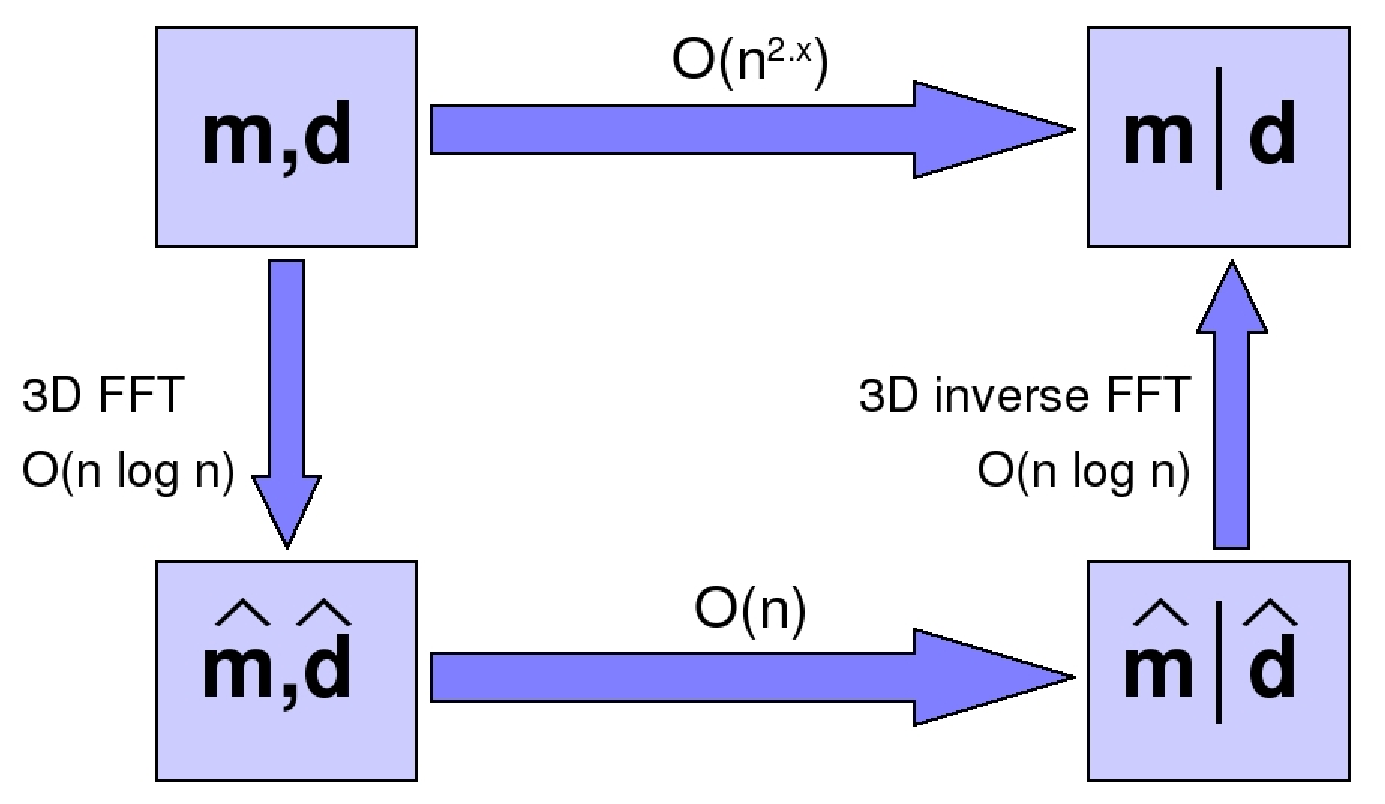
\includegraphics[width=.79\linewidth]{images/FFT_flowdiagram}
  \caption{The problem is transformed to the Fourier domain, solved
  in this domain, and back-transformed to time domain. This reduces
  the problem from a $\mathcal{O}(n^{2.x})$ to a $\mathcal{O}(n\log
  n)$ process.}
  \label{fig:FFT-flowdiagram}
\end{figure}


This seems to require that $\vect{d}$ is stationary, which would imply
that the wavelet must be the same everywhere. However, we can divide
out the wavelet from \autoref{eq:WADm} to obtain 
\begin{equation}
\label{eq:ADm}
\vect{d^\prime} = \vect{A}\vect{D}\vect{m} + \vect{e^\prime},
\end{equation}
where $\vect{d^\prime}$ is the data divided by the wavelet, and
$\vect{e^\prime}$ is the error divided by the wavelet. The details of
how we do this division is given in \autoref{sec:divwavimp}. Note that
we now assume that the noise after division, $\vect{e^\prime}$ is
stationary. Since we assume that a seismic response only depends on
the reflections in that trace, this division can be done trace by
trace. This assumption relies on a rather smooth seismic response, so
the lateral variations in the wavelet should be smooth. We have chosen
to restrict the local wavelet changes to only allow local temporal
shift and amplitude scaling. 

We can also work around the stationary noise assumption, and allow
$\vect{e^\prime}$ to vary laterally. This is done by utilising the
nature of a Bayesian solution, which always is a tradeoff between the
prior and the posterior with noise free data. By finding the posterior
for a minimal noise, we can then interpolate between this solution and
the prior to find an appropriate solution for the local noise
level. When doing this, we ignore the lateral correlation, so we
require constant noise level in each trace, since the conditional
correlations inside a trace are much stronger than between traces. See
\autoref{sec:localnoiseimp} for details. 

\subsection{Facies probabilities}
\label{sec:facprobthe}
To calculate facies probabilities from inverted elastic parameters we
must first establish a link between the elastic parameters from
inversion and facies. There are several ways to do this, and we have
listed the four most realistic in 
\autoref{tab:paramsfacies}.

First, we may establish the link using a rock physics models. This
way we avoid any alignment problems, but we get no frequency control
and get to use no correlation information from the
inversion. A prediction obtained this way tends to be too
optimistic, but if there are no well logs available, this is our only
option.

\begin{table}
\centering
\caption{Different methods for establishing a relation between elastic parameters and facies.}
\label{tab:paramsfacies}
\begin{tabular}{|l|l|l|l|l|l|}
\hline
Approach & Frequency & Inversion   & Alignment & Predictions\\
         & control   & correlation &  & \\ \hline
Rock physics                               &  No &  No & Yes & Optimistic  \\ \hline
Low-pass filtered elastic well logs        & Yes &  No & Yes & Optimistic  \\ \hline
Inversion                                  & Yes & Yes & No  & Pessimistic \\ \hline
Parameter filtered elastic well logs & Yes & Yes & Yes & Realistic   \\ \hline
\end{tabular}
\end{table}

Second, we may filter the elastic well logs using a low-pass filter,
and use these filtered logs and facies logs to make a density
estimation of $p(\bmu_{m|d_{obs}}|f)$, where $f$ is the facies. This
gives us frequency control and proper alignment, but again there are
no correlation information from the inversion included, and the
predictions become to optimistic. The frequency filtering of well logs
is illustrated in \autoref{fig:parmeterfilter}.

\begin{figure}
  \centering
  \fbox{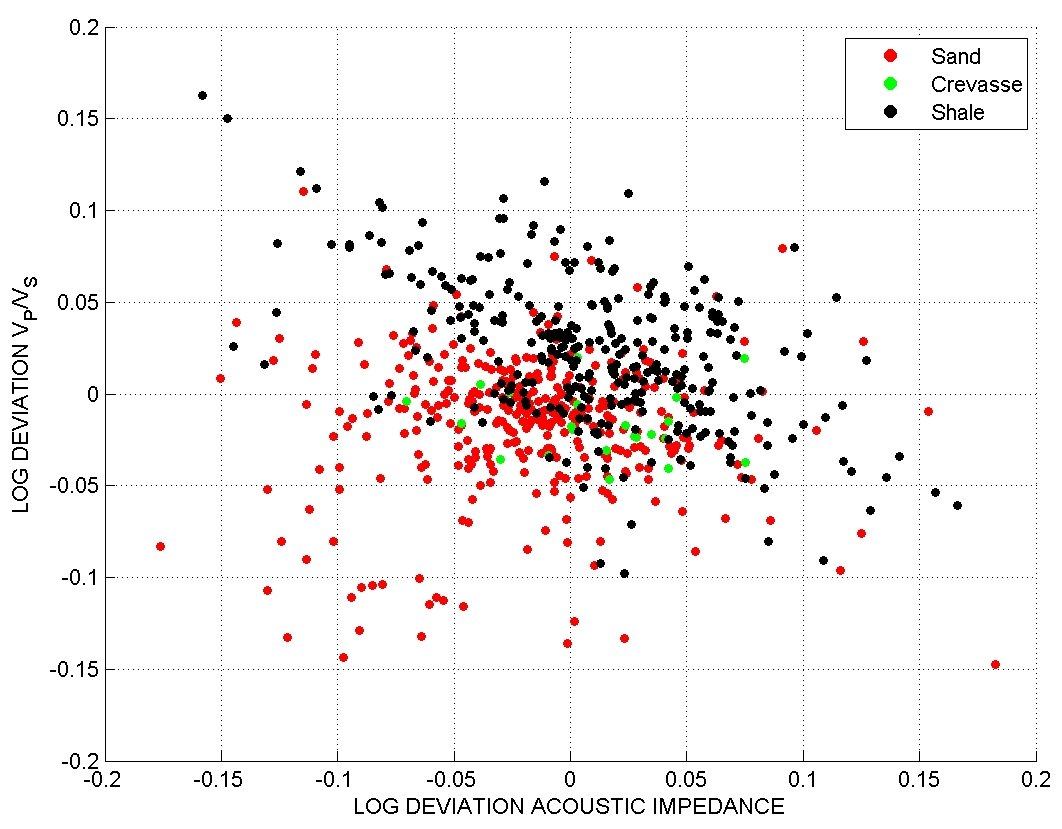
\includegraphics[width=.310\linewidth]{images/Crossplot_raw_logs}}
  \fbox{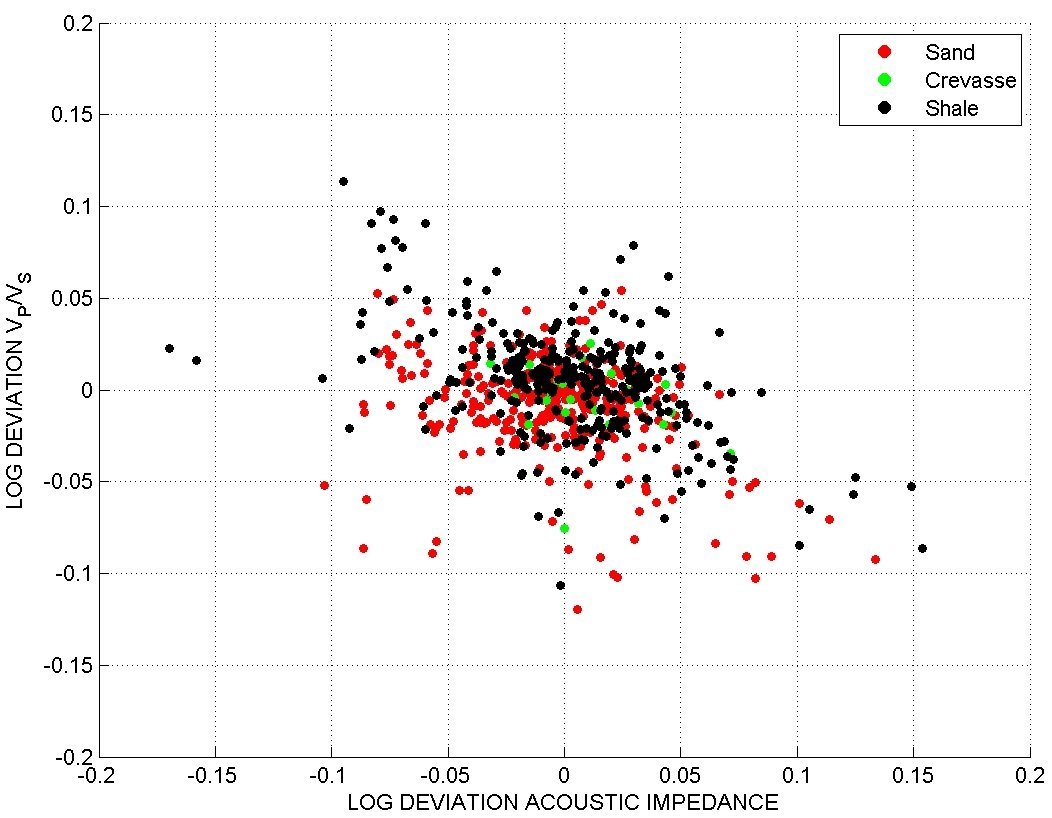
\includegraphics[width=.310\linewidth]{images/Crossplot_40Hz_logs}}
  \fbox{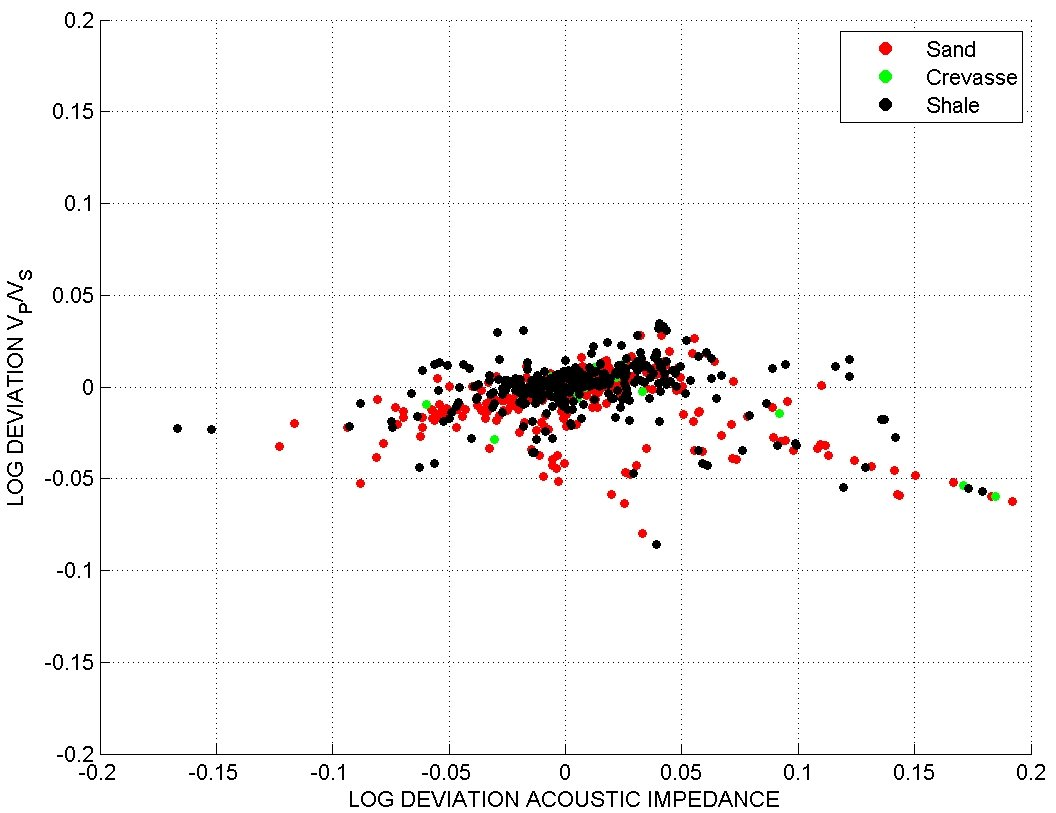
\includegraphics[width=.315\linewidth]{images/Crossplot_multi-parameter_filtered}}
  \caption{Acoustic impedance residuals calculated from blocked raw
    logs plotted against corresponding \vp/\vs  residuals (left), the
    same plot, but with logs high-cut frequency  filtered to 40Hz
    (middle), and the same logs but filtered using frequency and
    correlation information from inversion (right).} 
  \label{fig:parmeterfilter}
\end{figure} 

Third, we may set up the probability density for an elastic responds
given the facies directly from the inverted elastic parameters. This
way we get both frequency control and correlation information
included, but we get no alignment information, and the predictions
become to pessimistic.

Finally, we may establish the density using elastic parameters from
well logs, but filter these using frequency and correlation
information obtained from the inversion. Since we only use well logs
to establish the density estimates, we get no alignment problems, and
in total, this gives us realistic facies predictions. How the
inversion-based filtering differs from the pure frequency-based
filtering mentioned above is illustrated in
\autoref{fig:parmeterfilter}.  

The link between facies and elastic parameters that we eventually are
interested in is $p(f_i|\bmu_{m|d,i})$, where $f_i$ is the facies at
location $i$ and  $\bmu_{m|d,i}$ is the inversion result at the same
location. To establish this link, we must first establish a link
between the well logs $\vect{m}$ and the expectation given the seismic
data $\bmu_{m|d_{obs}}$. We get this 
by combining \autoref{eq:Gm} and 
\autoref{eq:mupost}: 
\begin{eqnarray}
\bmu_{m|d_{obs}} &=&\bmu_{m} +\bSigma_{m}\vect{G}^T \bSigma_{d}^{-1}
                           (\vect{d}_{obs}-\bmu_{d}) \nonumber \\
& = & \bmu_{m} +\bSigma_{m}\vect{G}^T \bSigma_{d}^{-1}
                           (\vect{G}\vect{m}+\vect{e}-\vect{G}\bmu_m) \nonumber\\
& = & \bmu_m + \vect{F}(\vect{m}-\bmu_m)+\vect{e}^*,
\end{eqnarray}
where
\begin{eqnarray}
\vect{F} & = &\bSigma_{m}\vect{G}^T \bSigma_{d}^{-1}\vect{G} \\
\vect{e}^* & \sim & \text{N}(0,\bSigma_{e^*}) \\
\bSigma_{e^*} & = & \bSigma_{m}\vect{G}^T \bSigma_{d}^{-1}\bSigma_e\bSigma_{d}^{-1}\vect{G}\bSigma_m.
\end{eqnarray}
The operator $\vect{F}$ is used to filter the well logs and obtain an
estimate of the expected inversion values $\vect{m}^\ast$. For each
facies, we then do a density estimation of $p(\bmu_{m|d_{obs}}|f)$ for
each possible facies value $f$ using $\vect{m}^\ast$ and facies
logs. The density estimation is done using a kernel smoothing
approach, and by using the distribution of $\vect{e}^*$ as our kernel,
we get an unbiased estimate of this distribution. 

Finally, we find the facies probability:
\begin{equation}
p(f=j|\bmu_{m|d_{obs}}) = \frac{p(\bmu_{m|d_{obs}}|f=j)p(f=j)}{\sum_i p(\bmu_{m|d_{obs}}|f=i)p(f=i)},
\end{equation}
where $p(f=i)$ is the prior probability of facies $i$. This
probability is then computed for each facies and each cell in the
grid, with $\bmu_{m|d_{obs}}$ given by the inversion results.

Far away from wells, the estimates will not be reliable, and we
introduce an undefined facies to show such areas. Denoting the
likelihood of this undefined facies $p(u)$, the facies probabilities
are now calculated as
\begin{equation}
p(f=j|\bmu_{m|d_{obs}}) = \frac{p(\bmu_{m|d_{obs}}|f=j)p(f=j)}{\sum_i p(\bmu_{m|d_{obs}}|f=i)p(f=i)+p(u)},
\end{equation}
where $p(u)$ is uniform over the area, and low compared to the
likelihood for facies when we are close to data. In
Figure~\ref{fig:faciesprobundef} the effect of the undefined facies in
a reservoir consisting of sand and shale is illustrated. The three
figures show cross plots of well observations of $\rho$ against \vp
combined with a probability map shown as a Colo coded map. 

\begin{figure}
  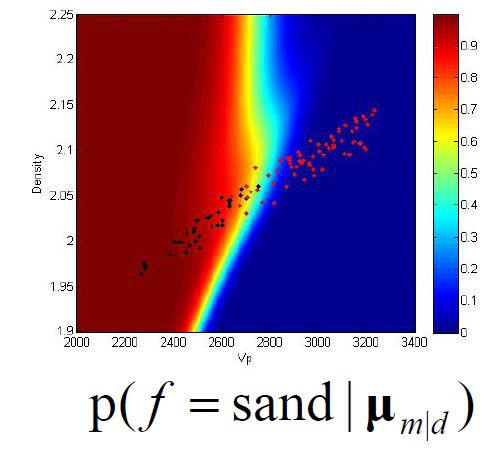
\includegraphics[width=.330\linewidth]{images/faciesprob1}
  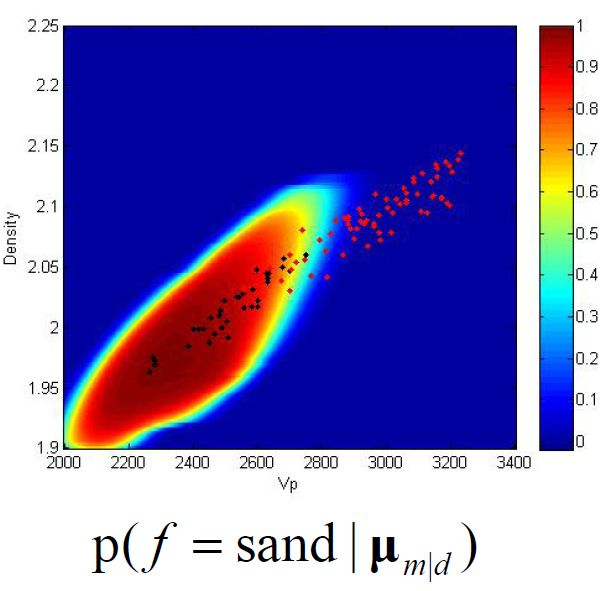
\includegraphics[width=.315\linewidth]{images/faciesprob2}
  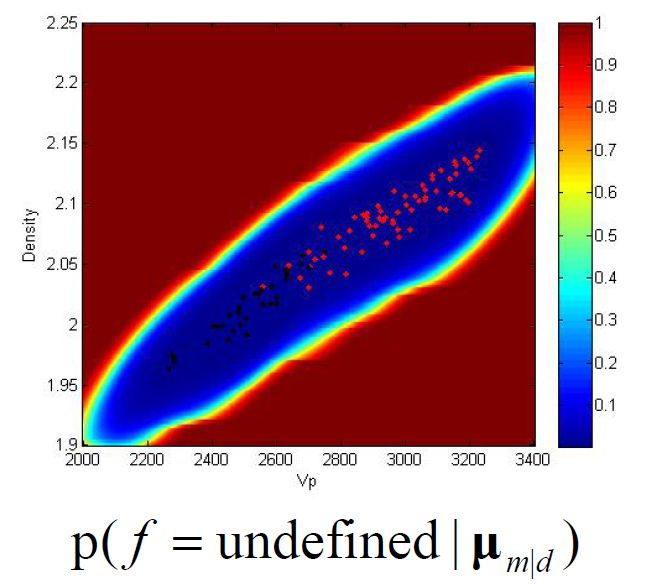
\includegraphics[width=.330\linewidth]{images/faciesprob3}
  \caption{To the left, the posterior sand probability calculated
    without undefined facies. In the middle, the sand probability when
    undefined facies is introduced. To the right, the posterior
    probability for undefined facies.}
  \label{fig:faciesprobundef}
\end{figure} 

In the left figure, we show the probability of sand before the
undefined facies has been introduced. Note how combinations of $\rho$
and \vp which are far away from any well observations, as for instance
(\vp, $\rho$) = (2000m/s, 2.25g/cm$^3$), may still lead to a facies
prediction of sand equal to one. This is not realistic.

In the middle figure, the undefined facies has been introduced, and
whenever we get far away from combinations of $\rho$ and \vp for which
we have no well observations, the probability for sand now decreases
to zero. This does not mean that there is no chance of finding sand at
the current spot, only that we have no data support to tell us what
facies we might find. Similarly, the probability of finding shale will
also be zero.

In the right figure, we show the probability of the undefined
facies. This is zero around well observations, and gradually increases
to one as the distance to observations increase. The probability of
shale may be extracted from these figures since
$p(\text{sand})+p(\text{shale})+p(\text{undefined})=1$.
